\section{Transmit Powers in a Wireless Network}

\textbf{(a)}

Let
\[
    D=\operatorname{diag}(G_{11},\ldots,G_{nn}),
    \qquad
    K=G-D.
\]
Here \(Dp\) is the vector of received signal powers, and \(Kp\) is the
vector of interference powers. The condition \(S_i=S^{\text{target}}\)
for every \(i\) is
\[
    G_{ii}p_i
    =
    S^{\text{target}}
    \left(\sigma+\sum_{j\neq i}G_{ij}p_j\right).
\]
In vector form this is
\[
    Dp=S^{\text{target}}\sigma\mathbf{1}
        +S^{\text{target}}Kp,
\]
or
\[
    (D-S^{\text{target}}K)p
    =
    S^{\text{target}}\sigma\mathbf{1}.
\]
Assuming \(D-S^{\text{target}}K\) is full rank, the only possible power
allocation is
\[
    p =
    (D-S^{\text{target}}K)^{-1}
    S^{\text{target}}\sigma\mathbf{1}.
\]
So the target SINR is achievable exactly when this \(p\) satisfies
\[
    0\leq p_i\leq P^{\max}, \qquad i=1,\ldots,n.
\]

\textbf{(b)}

\begin{figure}[h]
    \centering
    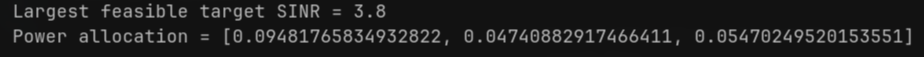
\includegraphics[width=0.7\textwidth]{img/7b.png}
\end{figure}

\begin{lstlisting}
using LinearAlgebra

G = [1   0.2 0.1;
     0.1 2   0.1;
     0.3 0.1 3]

sigma = 0.01
Pmax = 0.1
n = size(G, 1)

D = Diagonal(G)
K = G - D

best_S = nothing
best_p = nothing

for S in 2.0:0.1:4.0
    p = (D - S * K) \ (S * sigma * ones(n))
    feasible = all((p .>= 0) .& (p .<= Pmax))

    if feasible
        best_S = S
        best_p = p
    end
end
\end{lstlisting}


% These powers satisfy \(0\leq p_i\leq 0.1\). The next target,
% \(S^{\text{target}}=3.9\), gives
% \[
%     p =
%     \begin{bmatrix}
%         0.10188417523985663\\
%         0.05094208761992833\\
%         0.05935729973413477
%     \end{bmatrix},
% \]
% which violates the constraint \(p_1\leq 0.1\). Therefore \(3.8\) is the
% largest feasible target in the specified list.
